\chapter{Analisis}
\label{chap:analysis}

\section{Analisis Aplikasi Sejenis}
\label{sec:analysis-similarapps}

Untuk pembuatan perangkat lunak dalam skripsi ini, ada dua buah perkakas \cl yang akan diamati sebagai aplikasi sejenis, yaitu \chromewebstorecli dan \textit{iTunes Search API}.

\subsection{\chromewebstorecli\footnote{\href{https://github.com/pandawing/node-chrome-web-store-item-property-cli}{https://github.com/pandawing/node-chrome-web-store-item-property-cli}}}
\label{sec:similarapps-chromewebstore}

Perkakas \cl ini merupakan ekstensi dari sebuah aplikasi lain yang memiliki fungsi yang sama, yaitu \textit{Chrome Web Store Item Property}\footnote{\href{https://github.com/pandawing/node-chrome-web-store-item-property}{https://github.com/pandawing/node-chrome-web-store-item-property}}. Perangkat lunak \textit{Chrome Web Store Item Property} ini merupakan perangkat lunak yang akan memanggil fungsi API untuk mendapatkan metadata dari sebuah ekstensi pada \textit{web store} peramban Google Chrome. Perbedaan dari perkakas ini dengan aplikasi dasarnya adalah bahwa perkakas ini dapat digunakan sebagai perkakas \textit{command line}, sedangkan aplikasi dasarnya hanya bisa digunakan dalam perangkat lunak lainnya sebagai pemanggil fungsi API.

\subsubsection{Penggunaan}
\label{sec:similarapps-chromewebstore-usage}

Perkakas ini dapat digunakan melalui \textit{command prompt} dengan cara mengetikkan perintah sebagai berikut.

\begin{verbatim}
                     chrome-web-store-item-property <identifier>
\end{verbatim}

Dengan \verb|identifier| berupa ID dari ekstensi yang diinginkan. Jadi, misalkan pengguna memasukkan \verb|gighmmpiobklfepjocnamgkkbiglidom| sebagai ID yang akan digunakan sebagai \textit{identifier}, maka perkakas ini akan mengembalikan metadata dari ekstensi ``AdBlock'' sebagai keluarannya. Contoh penggunaan perkakas ini dapat dilihat di gambar \ref{fig:similarapps-chromewebstorecli}.

\begin{figure}[ht]
    \centering
    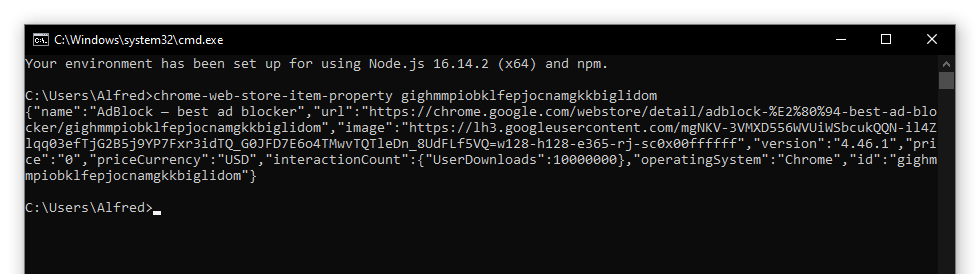
\includegraphics[width=0.75\linewidth]{chromewebstorecli}
    \caption[Contoh penggunaan perkakas \chromewebstorecli]{Contoh penggunaan perkakas \chromewebstorecli.}
    \label{fig:similarapps-chromewebstorecli}
\end{figure}

Sedangkan, keluaran dari perkakas ini merupakan sebuah objek JSON dengan properti-properti sebagai berikut.

\begin{itemize}
	\item \verb|name|\\
	Nama dari ekstensi yang dicari metadatanya.
	\item \verb|url|\\
	URL halaman web dari ekstensi yang dicari di \textit{web store} Google Chrome.
	\item \verb|image|\\
	Logo (dan ikon \textit{thumbnail}) dari ekstensi yang dicari metadatanya.
	\item \verb|version|\\
	Nomor versi dari ekstensi.
	\item \verb|price|\\
	Harga dari ekstensi. Jika ekstensi tidak memiliki harga yang perlu dibayarkan (gratis), properti ini akan bernilai \verb|0|.
	\item \verb|priceCurrency|\\
	Kode mata uang dari harga ekstensi. Jika ekstensi tidak memiliki harga yang perlu dibayarkan, properti ini akan berisi ``\verb|USD|``.
	\item \verb|interactionCount|\\
	Properti ini berisi interaksi-interaksi pengguna yang tercatat sebagai data di halaman \textit{web store} ekstensi. Pada saat pembuatan skripsi ini, properti ini hanya memiliki satu buah subproperti, yaitu \verb|userDownloads|, yang menandakan berapa kali ekstensi ini telah diunduh oleh pengguna di manapun.
	\item \verb|operatingSystems|\\
	Menandakan di peramban mana ekstensi versi ini dapat diinstal. Karena ekstensi-ekstensinya berada di \textit{web store} Chrome,
	\item \verb|ratingValue| (tidak digunakan lagi)\\
	Peringkat yang diberikan oleh para pengguna ekstensi ini. Nilai dari properti ini berupa skala desimal dari 0.00 sampai dengan 5.00. Di versi terbaru dari perkakas ini, properti ini tidak lagi tersedia dalam keluarannya.
	\item \verb|ratingCount| (tidak digunakan lagi)\\
	Jumlah pengguna yang telah menilai/memberi peringkat ke ekstensi ini. Di versi terbaru dari perkakas ini, properti ini tidak lagi tersedia dalam keluarannya.
	\item \verb|id|\\
	Properti ini mengandung ID dari ekstensi tersebut. Nilai dari properti ini akan sama dengan ID yang digunakan sebagai parameter masukan perkakas.
\end{itemize}

\subsection{\itunesapi\footnote{\href{https://github.com/awcross/itunes-search-api}{https://github.com/awcross/itunes-search-api}}}
\label{sec:similarapps-itunesapi}

Perkakas \cl ini berfungsi untuk melakukan pencarian melalui API iTunes, sehingga seakan-akan pengguna langsung melakukan pencarian di iTunes sendiri. Hasil pencarian yang dilakukan termasuk judul lagu, nama artis, ataupun nama album, dan pengguna dapat memilih secara spesifik objek apa yang ingin dicari.

\subsubsection{Penggunaan}
\label{sec:similarapps-itunesapi-usage}

Perkakas ini dapat digunakan melalui \textit{command prompt} dengan cara mengetikkan perintah sebagai berikut.

\begin{verbatim}
                      itunes-search-api <input> [<options>]
\end{verbatim}

Dengan \verb|input| berupa nama dari objek yang dicari. Perkakas ini juga memiliki opsi yang masing-masing memiliki parameter tersendiri untuk mempersempit hasil pencarian. Adapun opsi-opsi tersebut dapat dilihat di daftar di bawah ini.

\begin{itemize}
	\item \verb|country|\\
	\textbf{Kemungkinan nilai:} Kode negara dua huruf\\
	Opsi ini menerima parameter berupa kode negara asal dari album atau artis yang dicari.
	\item \verb|entity|\\
	\textbf{Kemungkinan nilai:} \verb|song|, \verb|musicArtist|, atau \verb|album|\\
	Menandakan jenis objek/entitas yang ingin dicari. Opsi ini dapat bernilai \verb|song| untuk pencarian berbasis judul lagu, \verb|musicArtist| untuk pencarian nama artis, atau \verb|album| untuk pencarian nama album. Jika opsi ini tidak dipakai, objek apapun yang memiliki kemiripan dengan \verb|input| dalam salah satu dari ketiga properti ini akan muncul dalam hasil pencarian.
	\item \verb|limit|\\
	\textbf{Kemungkinan nilai:} Bilangan bulat positif\footnote{Opsi ini juga menerima bilangan bulat negatif, tetapi menggunakan sebuah bilangan bulat negatif akan menghilangkan pengaruh opsi ini terhadap hasil keluaran.}\\
	Jumlah hasil pencarian maksimal yang ingin ditampilkan dalam keluaran.
\end{itemize}
\vspace{\baselineskip}
Sedangkan, keluaran dari perkakas ini merupakan sebuah objek JSON yang memiliki dua properti utama, yaitu:

\begin{itemize}
	\item \verb|resultCount|\\
	Properti ini berisi bilangan bulat yang menandakan berapa buah objek yang terdapat dalam hasil pencarian.
	\item \verb|results|\\
	\textit{Array} yang berisi kumpulan objek yang terdapat di dalam hasil pencarian. Objek-objek ini akan dikembalikan berupa sebuah \textit{array} lain yang berisi seluruh properti dari masing-masing objek. Apa saja properti yang diikutkan dalam \textit{array} tersebut tergantung tipe dari objek dalam hasil pencarian.
\end{itemize}
\vspace{\baselineskip}
Adapun contoh penggunaan dan hasil keluaran perkakas ini dapat dilihat di gambar \ref{fig:similarapps-itunesapi}.

\begin{figure}[ht]
    \centering
    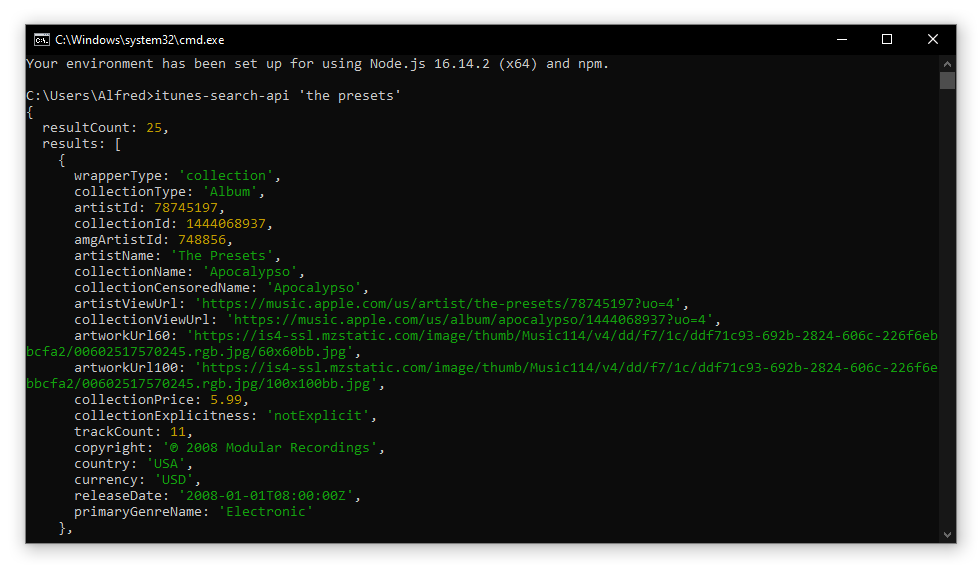
\includegraphics[width=0.75\linewidth]{itunesapi}
    \caption[Contoh penggunaan perkakas \itunesapi]{Contoh penggunaan perkakas \itunesapi. Gambar hanya memuat satu objek untuk menghemat tempat.}
    \label{fig:similarapps-itunesapi}
\end{figure}

\section{Analisis Modul dan Fungsi Bahasa C}
\label{sec:cmodules}

Di bagian ini akan dilakukan analisis terhadap seluruh modul dan fungsi dalam bahasa pemrograman C yang akan digunakan dalam pebuatan perkakas ini.

\subsection{getopt}
\label{sec:cmodules-getopt}

\verb|getopt| merupakan sebuah fungsi yang dapat mengautomasi pekerjaan-pekerjaan yang berhubungan dengan penerimaan opsi-opsi untuk \cl berbasis UNIX.\footnote{\href{https://www.gnu.org/software/libc/manual/html\_node/Getopt.html}{https://www.gnu.org/software/libc/manual/html\_node/Getopt.html}}
\newline\newline\noindent
Fungsi \verb|getopt| dapat dipanggil dengan format sebagai berikut.

\begin{verbatim}
                         getopt (argc, argv, <options>)
\end{verbatim}

Seluruh kode ini dapat dimasukkan ke suatu variabel berupa sebuah karakter yang merepresentasikan opsi yang ingin digunakan. \verb|argc| merupakan jumlah argumen yang terdapat dalam masukan, sedangkan argv merupakan sebuah \textit{array} yang berisi argumen-argumen tersebut.
\vspace{\baselineskip}
Selain itu, penggunaan \verb|getopt| juga memerlukan penggunaan variabel-variabel tertentu, yang dapat dilihat di daftar berikut.\footnote{\href{https://www.gnu.org/software/libc/manual/html\_node/Using-Getopt.html}{https://www.gnu.org/software/libc/manual/html\_node/Using-Getopt.html}}

\begin{itemize}
	\item \verb|opterr|\\
	Isi dari variabel ini akan memberi signal ke perangkat lunak/perkakas yang menentukan apakah \verb|getopt| akan mengirim pesan ke \textit{error stream} atau tidak. Jika variabel ini bukan bernilai 0, maka pesan \textit{error} akan dikirim. Sebaliknya, jika variabel ini bernilai 0, \verb|getopt| tidak akan mengirim pesan \textit{error} apapun, tetapi tetap akan mengembalikan sebuah karakter tanda tanya (\verb|?|) sebagai tanda bahwa sebuah \textit{error} telah terjadi.
	\item \verb|optopt|\\
	Ketika \verb|getopt| menemukan sebuah karakter yang tidak didefinisikan dalam kumpulan opsi, atau sebuah opsi yang tidak disertai argumen yang diperlukan, karakter tersebut akan disimpan di variabel ini.
	\item \verb|optind|\\
	Variabel ini digunakan oleh \verb|getopt| sebagai indeks untuk \textit{array} \verb|argv|. Jika seluruh argumen sudah diproses, nilai variabel ini dapat digunakan untuk menentukan argumen mana yang merupakan arguman tambahan yang tidak terpakai. Nilai dari variabel ini dimulai dari 1.
	\item \verb|optarg|\\
	Jika opsi yang sedang diproses memerlukan argumen, variabel ini adalah tempat dimana argumen tersebut akan disimpan.
	\item \verb|<options>|\\
	Variabel ini berupa \textit{string} yang menandakan karakter-karakter apa saja yang menjadi opsi yang mungkin dalam perkakas tersebut, beserta tipenya. Jika karakter opsi:
	
	\begin{itemize}
		\item Diikuti dengan titik dua (\verb|:|), maka opsi tersebut memiliki argumen yang bersifat wajib.
		\item Diikuti dengan titik dua ganda (\verb|::|), maka opsi tersebut memiliki argumen yang bersifat opsional.
		\item Tidak diikuti apa-apa, maka opsi tersebut merupakan opsi tidak berarguman.
	\end{itemize}
	
\end{itemize}

\subsubsection{getopt-long}
\label{sec:cmodules-getopt-long}

Ada pula versi \verb|getopt| yang memungkinkan perangkat lunak untuk menerima dua jenis opsi\textemdash opsi versi pendek berupa sebuah karakter singular, seperti pada \verb|getopt| biasa, dan/atau opsi panjang bergaya GNU, berupa sebuah kata.

\verb|getopt-long| juga memiliki seluruh variabel-variabel yang dimiliki oleh \verb|getopt|, hanya saja \verb|getopt-long| memiliki sebuah variabel tambahan berupa struktur, yaitu \verb|long_options|. Variabel ini merupakan sebuah struktur berupa \textit{array} yang berisi beberapa \textit{array} lainnya, di mana \textit{array-array} lain in merupakan masing-masing opsi dari fungsi \verb|getopt-long| tersebut. Tiap-tiap \textit{array} tersebut memiliki variabel-variabel berikut:

\begin{itemize}
	\item \verb|name|\\
	Variabel ini merupakan nama panjang dari opsi.
	\item \verb|has_arg|\\
	Variabel ini merupakan penanda apakah opsi memerlukan argumen atau tidak. Nilai yang mungkin dalam variabel ini adalah \verb|no_argument|, \verb|required_argument|, atau \verb|optional_argument|.
	\item \verb|flag| \& \verb|val|\\ 
	Kedua variabel ini menandakan bagaimana sebuah opsi akan diberlakukan ketika diterima oleh \verb|getopt-long|. Variabel \verb|flag| dapat diisi dengan penunjuk ke suatu variabel lain yang akan diisi dengan isi dari variabel \verb|val| untuk menandakan bahwa \verb|getopt-long| telah berhasil memroses opsi tersebut. Di lain sisi, jika variabel ini berisi \textit{null pointer}, maka fungsi \verb|getopt-long| akan mengembalikan isi dari variabel \verb|val|.
\end{itemize}
\noindent
Struktur ini harus diakhiri dengan sebuah \textit{array} tambahan yang seluruh variabelnya bernilai 0.

\section{Analisis API KIRI}
\label{sec:kiri-analysis}
